\chapter{Ludmila Zahradnik}

Lady Shalltear’s attendants piled the books and files that they had carried all the way from the guest house – as well as those they retrieved from the floor after Aemilia had fainted – on the counter, quietly returning to their mistress’ side without a word or even hint of complaint. The Undead clerk they were placed in front of looked to the stack and back to them again, while the seven others turned their heads to watch the proceedings. Even if they had been human officials, Ludmila felt that all of this scrutiny would have felt fairly awkward.

 

Standing aside while the attendants dropped off her things at the desk, Ludmila asked a question.

 

“Lady Shalltear, what sort of Undead are these?”

 

“They’re Elder Liches,” Lady Shalltear answered.

 

“The same Elder Liches as the ones in the forms?”

 

“If the forms say ‘Elder Liches’, then I suppose that would be the case.”

 

It occurred to Ludmila that Lady Shalltear had not actually read all of the paperwork that she herself had spent hours poring through since the previous evening. Her liege did not miss the put-upon look that she gave her.

 

“W-we have plenty of them wandering about,” Lady Shalltear told her as she gestured about loosely with her left hand, “and they’re smart enough for the Guardian Overseer to have a small army of them trained to be ready for administrative tasks soon. Unfortunately, they haven’t had a chance to prove themselves, so they’ve understandably become quite restless – just look at how eager these ones are.”

 

In front of them, the crimson points of light in the hollows of the Elder Lich’s skull flared. It could have been angry, excited, happy or bored for all Ludmila could tell. Aemilia whimpered from behind, and Ludmila turned to speak to her.

 

“Luzi,” she said in soothing tones, “if you are still a bit uncomfortable around the Undead, you may rest in the waiting area with Lady Shalltear’s attendants while she and I attend to business.”

 

Lady Shalltear, face painted with the realization that her attempted deflection had failed, piped up in a surprised voice.

 

“Wait, why am I doing this as well?”

 

“A lady of your station should have an understanding of the inner workings of the realm, should she not?” Ludmila asked.

 

“I told you, I’m really only good for fighting…” Lady Shalltear looked down and brought the points of her fingers together.

 

“I do not believe that,” Ludmila said, “I think you are an excellent mentor, my lady. You have already helped me far beyond my expectations, including with things I never would have conceived of before – you are a font of wisdom, and you possess charisma that any noble would envy.”

 

“The Sorcerer King has other subordinates that are much smarter than me, you know?”

 

For some reason, Lady Shalltear seemed to not harbour much confidence in herself. Ludmila could not understand how such an amazing woman could have such a self-deprecating disposition.

 

“Those with the gift of intellect surely play a crucial role in the workings of a realm,” Ludmila agreed, “but it is wisdom that guides, and charisma that leads. When the peoples’ hearts are troubled; when souls in turmoil seek stability, they turn not to the sages with their inventions and ideas, but to trusted elders and dependable priests. When faith is kindled and loyalty inspired, it is more often achieved by the words of a great orator than it is the result of some clever scheme. It may be as you say and you cannot match the intellect of some of your peers but, personally, I think your other qualities more than make up for it.”

 

Both of Lady Shalltear’s appearances held equally complicated expressions upon hearing Ludmila’s words. Whatever her inner conflict was, however, it ended abruptly when she brought her palms up to slap her cheeks loudly.

 

“Ei! Fine, I’ll do it.” Her expression looked like she was preparing to go to battle rather than submitting paperwork, “I’ll have you explain things to me if I have any questions about this…”

 

“It would be an honor to serve, my lady,” Ludmila lowered her head.

 

Lady Shalltear turned to her attendants and waved them away. They, together with Aemilia, left to wait back near the front windows of the office. Ludmila watched as they seated themselves together in a small circle of chairs, facing one another.

 

“I have been wondering for a while now…your attendants, are they your Acolytes?” Ludmila asked, “Or perhaps is that how maids dress where you hail from?”

 

“They’re my Vampire Brides,” Lady Shalltear answered. “I have many of them under my authority, and they serve as my attendants in…various ways.”

 

Ludmila looked back towards the waiting area at Aemilia, who seemed to be trying to strike up a conversation with the silent attendants without much success.

 

“They are silent most of the time,” Ludmila noted. “Do they speak much on their own?”

 

“Why of course,” Lady Shalltear said. “They can be quite talkative. Out here, however, there’s usually not much reason for them to say anything.”

 

“…I see.”

 

Aemilia would be in for quite a shock if she inadvertently discovered that she was trying to chat with the very Undead that she was deathly afraid of. Ludmila hoped she would come back to a conscious servant when she finished with her work here.

 

The clerk’s withered face betrayed no sign of irritation or impatience at the continuous delays as the pair stepped up to the counter. Ludmila instinctively tested the air at the sight of its desiccated flesh but, rather than the stench of decaying corpses, there was a very faint trace of the cold, unsettling scent that was associated with the Undead. With so many of them in the city, she was surprised that she had not really detected this before now – it must have been the enclosed space of the office that allowed the odour to collect and linger in the air.

 

They seated themselves on the tall, cushioned stools that were lined up in front of the reception counter and Ludmila reached for the folder at the top of the pile laid upon it. Fishing out the application forms that were in various stages of completion, she skimmed through them one last time before pushing the first completed application forward over the counter.

 

A shriveled hand reached out and held the form upright as the Elder Lich briefly scanned the piece of paper. It then wordlessly held up the form beside its head. From above, there was a leathery flutter as an Imp swung down from its perch, swooping over their heads as it snatched the form and flew away deeper into the office.

 

The hand lowered to rest on the counter once again and the Elder Lich resumed staring at Ludmila.

 

“...that’s it?” She stared back blankly.

 

“I-I didn’t understand any of that,” Lady Shalltear said from beside her with a distraught look. “I told you I was only good for fighting. Maybe I should quit while I have some dignity left?”

 

Ludmila presented the next form. Only two had been completed, while the rest lacked various degrees of crucial information. The first was a request for agricultural labour for the old terraces where she planned to cultivate oats. This one was for harvesting timber.

 

Again, the process repeated itself. Though the first Imp had not returned yet, a second from the neighboring counter took the form away. The next form – for road construction – was nearly complete, but it required a director to oversee the labour. She laid the sheet on the counter between them.

 

“I would like to request a…technical advisor for road construction,” Ludmila said.

 

The Elder Lich lifted the sheet, scanning it in the same manner as the previous forms. This time, it set it back down on the counter before speaking in a deep voice that sounded like someone was rubbing two pieces of dried leather together.

 

“There are currently no technical advisors for this request available,” it said. “The current waiting time is…undefined.”

 

Ludmila blinked several times. She turned her head to look at Lady Shalltear, who seemed to be busy trying to read the upside-down form, then back at the clerk.

 

“Does that mean I have to find my own advisor?” She asked.

 

“All requests must be fulfilled through the central administration,” the Elder Lich replied. “Technical advisors must be trained and licensed for operations by the Department of Transportation and Logistics.”

 

“Oh, that’s me…I think?” Lady Shalltear spoke in what sounded like half a question beside Ludmila.

 

“The Minister of Transportation isn’t familiar with her Department’s own paperwork?” Ludmila asked.

 

Ludmila tried ignoring the fact that Lady Shalltear appeared to be surprised by her own realization that she was the Minister of Transportation. She wondered if the reason why the Elder Liches were all paying such close attention to them was that they thought they were being tested by a member of the King’s Cabinet.

 

“There’s so much of it, and it just came out at the beginning of the week,” Lady Shalltear said in an attempted defence, “besides, my Vampire Brides are capable of handling most of the paperwork.”

 

“Still…you are the department head, are you not, my lady?” Ludmila said, “Making sure that everything runs smoothly and that appropriate policies are passed in the Royal Court is a duty appointed to you by His Majesty, is it not?”

 

“Argh, I get it already! I’ll take a look at all this at night while you’re sleeping. Let’s just get on with the rest of what you have here.”

 

“Do you know of a technical advisor for this form, my lady?” Ludmila asked.

 

“Isn’t that part of what you’re supposed to be helping us out with?” Lady Shalltear answered, “Just find some and bring them to me; I’ll sign off on it.”

 

“The Elder Lich said they have to be trained and licensed first.”

 

“It will be on site training! We can use your request for it, then use the trained advisors to help recruit and train new advisors.”

 

Ludmila supposed she would have to find someone familiar with planning and directing road construction, as she had no such expertise. She took back the form for road work and pulled out the next.

 

“I have questions about this form–”

 

“The forms have been approved for official use by the Guardian Overseer,” the Elder Lich interrupted her. “Compliance is mandatory.”

 

The tone of finality in the clerk’s words gave Ludmila pause. Recalling that these clerks were in reality powerful Undead mages, she wondered if non-compliance resulted in a hapless petitioner being immolated in their seat. She resisted the urge to check the carpet for scorch marks as she rephrased her request.

 

“I require clarification on some of the fields within this form,” she said carefully.

 

Reaching under the counter, the Elder Lich pulled out a tome that looked identical to those that she had been provided by Yuri Alpha. It rapidly flipped through the pages, mechanically coming to a stop at exactly the right section. Ludmila leaned over to point out various parts of the page.

 

“As you can see,” she said, “there are no recommendations for this produce listed in the almanac. Many of the goods harvested in my fief grow in marshes and wetlands, and there are no similar references to use.”

 

“For fields not specified by reference materials,” the Elder Lich said, “collection of data is prescribed. State your request.”

 

“To begin with, I would like to know what these ‘units of labour’ mean. What is a ‘light unit’?”

 

“A light unit of labour is a single undead servitor, rated from level one to twenty.”

 

Undead? Level? In hindsight, Ludmila thought she shouldn’t have been surprised at the first revelation, but was completely oblivious about the rest.

 

“What is a…‘level’?” Her mouth worked slowly around the unfamiliar word.

 

“A level is a measure of your proficiency in a class,” Shalltear said from beside her, “I believe your Adventurers use something similar, but less concrete and subject to the reporter when estimating the strength of individuals.”

 

“What is a ‘class’, my lady?” Ludmila wasn’t sure she understood, “Does it have something to do with one’s vocation?”

 

“...not quite.” Lady Shalltear said, “A person may have classes outside of those related to their current vocation. Just think of it as getting better in what you’re doing, and growing in physical ability. In the case of a combatant, it also means that they gain access to more powerful spells and attacks. The civilian classes here may also have something along those lines related to their own matters.”

 

Lady Shalltear’s rough description made at least some sense to Ludmila, but she had never heard of natural growth and learning phrased in those exact terms. Adventurers recognized their own along similar terms and clear measures of power could be defined amongst practitioners of magic.

 

“I see,” she said. “Then what would an example of a ‘light unit of labour’ be?”

 

Lady Shalltear spun in her chair, facing the open chamber behind them, prompting Ludmila to turn as well. A line of Undead creatures materialized and rose before them. Ludmila had Skeletons or Zombies in mind, but there were quite a variety that she had not thought of or seen before.

 

“The Skeleton Warriors like the ones I summoned yesterday were level sixteen – there are different types as well, but I’m not sure exactly which kind you’d be getting for this sort of menial labour. Those humanoid Zombies…well, it’s probably a bad idea to use them. There are a few that I don’t think you’ll find much use out of, like the Vampire Bats and Incorporeal Undead.”

 

Shalltear made a waving motion, after which many of the Undead presented disintegrated into the air. There were several remaining: mostly Skeletons and a handful that had the appearance of animals.

 

“Undead Beasts are Zombie-types,” she continued, “but exhibit some of the qualities of the animals that they emulate. The cute puppy there that looks like a black wolf is level seven and may be used in much the same way as a hound...I’m unsure if those will be made available. The rest are anywhere between one to twenty, like the ones provided by the administration.”

 

“Is that one an Undead Beast, or a Skeleton?” Ludmila pointed to one of the only Undead summons remaining that looked like it could fly.

 

“That’s a Bone Vulture,” Lady Shalltear said, “it’s a Skeleton-type. The Vampire Brides that follow me around are in the low twenties…if you need one of them to help with something that requires intelligence, I can assign them to you directly.”

 

Having the various Undead displayed before her like they were varieties of livestock felt a bit surreal. Ludmila was long over feeling like a fish out of water, however. She turned back to the counter to look at her forms.

 

“Any combination of these Undead is available for request?” She asked the clerk.

 

“For industrial purposes, yes,” the Elder Lich answered. “Undead servitors that can spread disease, wither the living with negative energy and those that have no suitable applications in industry are prohibited.”

 

Ludmila ran some figures in her head based on the recommendations for the other goods she had submitted, filling out the remaining blank spaces on the forms. Lady Shalltear watched from beside her as she went from document to document.

 

“What about these ‘heavy units of labour’?” Ludmila asked.

 

“Death Knights are employed to operate larger pieces of equipment,” the Elder Lich told her, “as well as perform other types of heavy labour. Soul Eaters are used to transport goods – a vehicle is not included.”

 

Ludmila continued marking out the forms.

 

“What about these ‘special construction units’?”

 

“Golems for large-scale development projects,” the clerk responded. “The palisade constructed around Carne Village is an example of their use.”

 

There were hundreds of villages in the duchy, and Ludmila had never heard of this particular one before. Why a village would merit such fortifications, she had no idea. She continued working through the forms.

 

“Golems aren’t Undead, are they?” Ludmila asked.

 

“Golems are Golems,” the Elder Lich replied flatly.

 

“Constructs,” Lady Shalltear offered helpfully.

 

The horses used by Darkness were the only Golems Ludmila had ever seen, so she was curious what they looked like. She hardly thought it appropriate to request one for just that reason, however. She would have to wait until she had a need for them. Filling out the last of the industrial forms, she handed them in all at once. As the clerk went through her submissions, Ludmila turned to speak to Lady Shalltear.

 

“These Undead will fight if instructed to, my lady?” She asked, “Say…if the village is raided by Demihumans.”

 

“Of course,” Lady Shalltear answered. “Their original purpose is to fight according to their summoner’s will, after all.”

 

“What ‘level’ are Death Knights?”

 

“They’re level thirty-five – oh, they're actually stronger than a regular Death Knight since they're enhanced by His Majesty’s abilities.”

 

The numbers started to become ambiguous. Skeleton Warriors like the ones summoned by Lady Shalltear would rarely appear on the Barony’s shores when the wilderness tribes had particularly large conflicts upriver, but a solid patrol could work together to destroy one safely.

 

“Does that mean they are twice as strong as Skeleton Warriors?” She asked.

 

“Oh, no,” Lady Shalltear replied. “Double the level does not mean double the strength.”

 

“Then what is a Death Knight capable of?” Ludmila said, “In the past, some of the raids along the border have been very strong – especially if they involved some important rite for a prominent Demihuman warrior, or a desperate attack in hard times to secure resources.”

 

Lady Shalltear tapped her lip with a finger as she mulled over the question.

 

“Well, you requested five Death Knights,” she said at some length. “That should have been enough to kill everyone in the city of E-Rantel – under Re-Estize’s rule – within a day or two if there weren’t many strong Adventurer teams present to defend the walls. They’d be quite effective at cleaning out the city districts with their special ability.”

 

“Erm…I suppose that should be good enough then.”

 

“Perhaps,” Lady Shalltear said noncommittally, “I’ve no idea how strong your Demihumans are, but if your people have successfully kept them at bay, then I’d say that you’d be correct.”

 

Ludmila put away the military request forms. There shouldn’t be a need for excessive force. If she requested too many, she might come under suspicion for belligerent intentions.

 

“And what of me, my lady?” She finally asked, “What ‘level’ would you say I am?”

 

Lady Shalltear peered at her for a moment before answering.

 

“If Aura was here she might be able to give you a better estimate, but based on how tough you appear to be compared to various Adventurers and city militia…level three?”

 

Ludmila sighed. It seemed that every single member of her future workforce could soundly thrash her. She hoped that she would be able to manage them properly.

\begin{figure}
    \centering
    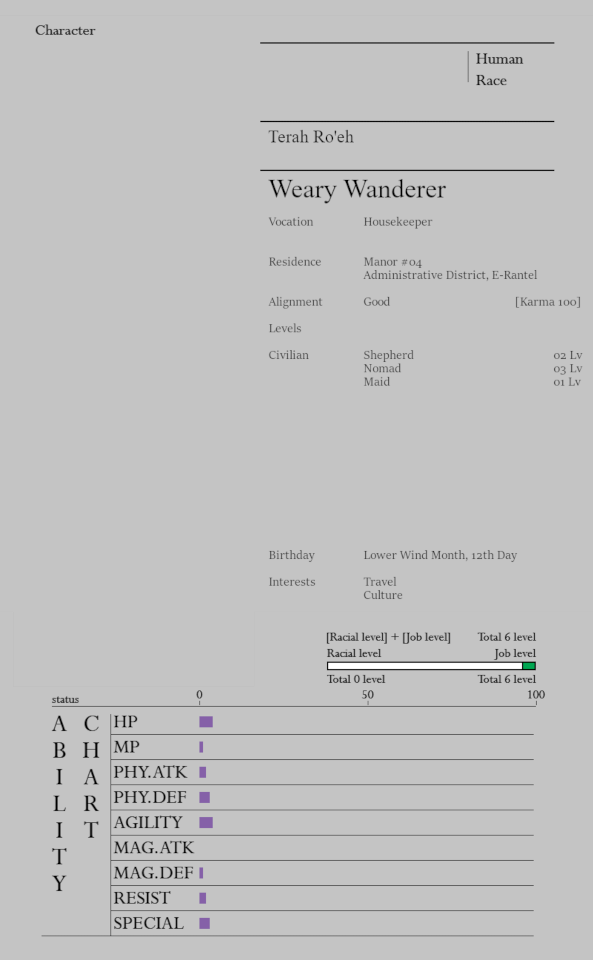
\includegraphics[width=1\linewidth]{V1 Birthright//images/8ugC7a1.png}
    \caption*{Terah Ro'eh Character Sheet}
\end{figure}


\section*{The Noble Household (Part II)}

Those women serving in domestic matters within a household – colloquially termed ‘maids’ – cover a wide range of specialized roles with varying degrees of importance and authority.

 

Housekeepers are managers over the majority of the women serving in these domestic tasks, reporting directly to the lady of the house. They are responsible for hiring, development and promotion of those working under them and the overall condition and appearance of the manor. It is a senior position in the household retinue, and a Housekeeper is usually served by junior members of the staff.

 

A Lady’s Maid is a direct attendant of the lady of the house. They assist in managing their mistress’ wardrobe and appearance, as well as see to their various personal needs. Like the Housekeeper, it is a senior position in the household retinue and does not normally see to menial tasks that junior positions are responsible for. Though a Lady’s Maid also reports directly to the lady of the house, the Housekeeper holds authority over the rest of the female staff, and indirectly outranks her. A Lady’s Maid is not to be confused with a Lady-in-Waiting: a companion of noble birth who serves in a similar capacity.

 

Those most closely associated with the common perception of maids are the junior staff, each performing specific duties in their part of the manor. Maids who work ‘upstairs’ attend to tasks in the private areas of the manor. Those who work ‘downstairs’ tend to the common areas of the manor, usually on the main floor or storage areas. The grades delineating their positions in the household hierarchy is usually dependent on the nature of the work itself – those assigned to the most menial tasks tend to be the least respected and subjected to the worst conditions.

 

It should be noted that maids performing kitchen duties do not report to the Housekeeper, but to the Cook.